\chapter[LWFA Bremsstrahlung Source for linear BW]{Characterisation of a LWFA Bremsstrahlung Source for a Measurement of the Linear Breit-Wheeler Process}
\label{Chap:BW}

\section{Motivation and Introduction}

The Breit-Wheeler process is the inverse process of the more commonly observed Dirac annihilation \cite{Dirac1930_Annihilation}, where an electron and a positron decay into two photons \cite{BreitWheeler1934_BW}. In the Breit-Wheeler mechanism, two (linear) or more (non-linear) photons combine to produce an electron-positron pair --- in other words matter is created from light. The linear Breit-Wheeler process is the simplest mechanism by which photons can create matter and is one of the most fundamental interactions of quantum electrodynamics (QED) that can be represented by minimally-sized Feynman diagrams (see Figure \ref{BW:Figs:OPike_TreeDiagrams}). However, despite its simplicity it is the last of these fundamental interaction that has not been definitively observed in isolation in vacuum, i.e. without the presence of other particles or external fields. Its measurement is particularly relevant for the field of high-energy astrophysics \cite{Nikishov1962_PAIRSASTRO,Bonometto1971_PAIRSASTRO,Ruffini2010_PAIRSASTRO}.
\vspace{\baselineskip}

The non-linear Breit-Wheeler process, on the other hand, has been measured and confirmed previously as part of the E144 experiment at SLAC in the `90s where an ultrarelativistic electron beam of $46.6\,\mathrm{GeV}$ energy was collided with an intense laser pulse $a_0 \sim 0.3$, resulting in highly energetic gamma photons from inverse Compton scattering \cite{Bula1996_RR,Burke1997_RR}. These gamma photons in turn interacted with up to $n \approx 7$ laser photons to produce electron-positron pairs \cite{Hu2010_TRIDENT}. The researchers detected about 100 positrons that match the momentum profile for products from the non-linear Breit-Wheeler and the Trident process \cite{Ilderton2011_TRIDENT} over the course of 22,000 laser shots.

The measurement of other photon-photon interactions, elastic and inelastic scattering processes, is additionally very challenging as these are higher order processes with cross sections that are suppressed by at least $\sim \alpha^{-2}$. As a result similarly few events have been measured for other photon-photon interactions without background fields, for instance at the Large Hadron Collider (LHC): the ATLAS collaboration reported on 13 candidate events for light-light scattering in heavy-ion collisions \cite{ATLAS2017_GammaGamma,dEnterria2013_GammaGamma}. The OPAL Collaboration at LEP, on the other hand, measured inelastic photon-photon interactions \cite{OPAL2000_GammaGamma}.
\vspace{\baselineskip}

\begin{figure}
\centering
\includegraphics[width=.9\columnwidth]{QED_TreeDiagrams_OPike.jpg}
\caption[Overview of theoretical fundamental QED processes shown in their Feynman representation along with the year the process was validated experimentally.]{Overview of theoretical fundamental QED processes shown in their Feynman representation along with the year the process was validated experimentally. Each of the processes has been observed in experiment, with exception of the Breit-Wheeler pair production, and either theoretical or experimental work related to them has been rewarded with a Nobel prize. Figure made by Oliver Pike, accessible at REF PHYS ORG URL.}%https://phys.org/news/2014-05-scientists-year-quest.html
\label{BW:Figs:OPike_TreeDiagrams}
\end{figure}

Pair annihilation is easily measured in radioactive decays \cite{Klemperer1934_Annihilation} as its cross section is very high at low energies ($\sigma_{e^+ e^-} \propto 1/E$) and an abundance of electrons in ordinary matter provides an abundance of attractive partners for positrons to annihilate with. Pair creation from radiation, on the other hand, requires high energy photons and/or a very high photon density, for instance a tightly focused laser, to overcome the production threshold in the centre-of-mass frame:

\begin{equation}
\boxed{s = \frac{E_1 E_2}{2m^2_e c^4} (1-\cos\theta) > 1,}
\end{equation}

where $s$ is the centre-of-mass energy, $E_1,E_2$ the energy of the first and second photon, respectively, and $\theta$ is the angle between the two photons.
Any excess energy can provide the created pair with sufficient momentum to avoid an immediate decay through Dirac annihilation. The quantities of the Breit-Wheeler and annihilation total cross-sections are related by $\sigma_{\gamma \gamma} = 2\beta^2 \sigma_{e^+e^-}$, where $\beta = \sqrt{1-1/s}$ (see Figure \ref{BW:figs:BW_Dirac_Xsec}).
However, delivering two bright photon sources at suitable energies at the same location is very challenging and hence mainly mediated pair production processes in presence of a background field have been measured instead \cite{Bethe1934_BH,Heitler1954_BH,Gahn2000_BH,Chen2009_BH,Sarri2013_pairs,Sarri2015_pairs,Bula1996_RR}. 
\vspace{\baselineskip}

\begin{figure}
\centering
\includegraphics[trim={5.0cm 0 6.0cm 0}, clip, width=1.0\columnwidth]{BWD_Xsec.png}
\caption[Breit-Wheeler and Dirac cross-section.]{Breit-Wheeler and Dirac cross section as function of the centre-of-mass energy $\sqrt{s}$. For $s\rightarrow 1$ the pair production cross section falls to zero whilst the annihilation cross section diverges. The maximum value of the Breit-Wheeler cross section coincides with the energy at which both cross sections are equal.}
\label{BW:figs:BW_Dirac_Xsec}
\end{figure}

Directed high energy radiation in the $\mathrm{keV}$ range can be produced from highly relativistic electrons, for instance at XFELs and synchrotron sources using bending magnets and insertion devices, and equivalently in plasma accelerators through betatron radiation \cite{Rousse2004_BETATRON,Kneip2010_BETATRON}. Another approach is to sufficiently heat solid targets with a laser, for instance hohlraums \cite{PikeThesis} or burn-through foils \cite{Edwards1990_BURNTHROUGH}.

Directed energetic gamma radiation can be generated by passing highly relativistic electrons through solid material to produce bremsstrahlung \cite{Glinec2005_Brems} or relying on inverse Compton scattering \cite{Sarri2014_ICS,Yan2017_ICS}.
\vspace{\baselineskip}

\begin{figure}
\centering
\includegraphics[width=.7\columnwidth]{OPike_nphoton_plot.JPG}
\caption[Experimental setup for a photon-photon collider as proposed by Pike et al.]{Experimental setup as proposed by Pike et al. in \cite{Pike2014_BW}. Figure 1 in \cite{Pike2014_BW} reprinted by permission from Nature Photonics, copyright (2019).}
\label{BW:figs:PikeSetup}
\end{figure}


In 2014, \textit{Pike et al.} \cite{Pike2014_BW} proposed to measure the linear Breit-Wheeler process by combining a low-divergence ($\theta \sim \ln(\gamma)/\gamma$ \cite{Stearns1949_Brems}) bremsstrahlung source, consisting of a GeV-class electron beam generated by a high-intensity laser\cite{Leemans2006_GEV}  and a gold foil \cite{Glinec2005_Brems}, with a blackbody radiation field formed in a hohlraum heated by a high-energy laser (see Figure \ref{BW:figs:PikeSetup}) \cite{Lindl2004_HOHLRAUMBASICS,Decker1997_HOHLRAUM,Town2011_HOHLRAUM,Glenzer2011_HOHLRAUM}. For $10^9$ electrons at 2 GeV energy, a 5 mm thick gold foil and a 1-cm long hohlraum at temperature of 400 eV, the researchers predicted up to $10^5$ pairs to be generated from the linear Breit-Wheeler process. The asymmetry of the energies produced by the two photon sources results in an emission of pairs in the direction of the higher energetic gamma ray beam. This is referred to as pair beaming \cite{Ribeyre2018_BW}, which in principal allows the extraction and measurement of all pairs produced, better separation of signal and noise, and using smaller detectors.
The setup also opens up the possibility to investigate elastic photon-photon scattering of the gamma-rays in the X-ray field \cite{dEnterria2013_GammaGamma}.

\begin{figure}
\centering
\includegraphics[width=.7\columnwidth]{2018QED_Chicane.JPG}
\caption[In pursuit of creating matter from light. Photograph of the magnetic chicane.]{In pursuit of creating matter from light. Photo taken during the experiment campaign aimed at measuring the linear Breit-Wheeler process at the Gemini facility in 2018. View upstream on the gamma-ray axis, indicated by a green alignment laser, through the magnetic chicane that is designed to transport generated electron-positron pairs from the Breit-Wheeler process to designated single particle detectors.}
\end{figure}

The experiment presented here is based on this proposed layout \cite{Pike2014_BW,PikeThesis}: two lasers are employed to provide simultaneously an X-ray and a gamma-ray source to overcome the mass threshold and to produce electron-positron pairs from the linear Breit-Wheeler process. A detailed description can be found in Section \ref{BW:sec:expSetup} (see also Figure \ref{BW:fig:exp_sketch}). The gamma rays are produced, as proposed, by bremsstrahlung from LWFA electrons \cite{Glinec2005_Brems}, but in this instance typically at electrons energies $\epsilon_{e^-} < 1\,\mathrm{GeV}$. As converter the higher-Z metal bismuth (Bi) is used which allows reducing the material thickness with respect to the proposed gold foil at comparable conversion efficiency, but at lower maximum cut-off energy. Instead of using a high-energy laser and a hohlraum, a replenishable burn-through foil germanium target in conjunction with another high-intensity laser is used \cite{Edwards1990_BURNTHROUGH}, producing an X-ray spectrum with emission lines peaked around $1.5\,\mathrm{keV}$ (REF). This balances out the lower gamma-ray energy and a narrow bandwidth spectrum constrains the interaction conditions.
Using a replenishable foil target and a high-intensity instead of a high-energy laser also allows making use of high repetition rate systems.
By removing the X-ray target from the beam axis we also reduce the production of secondary Bethe-Heitler pairs from gamma rays interaction with solids that might be mistaken for pairs produced in the linear Breit-Wheeler process.

\section{Chapter Outline}

This Chapter relates to an experimental campaign aimed at measuring the linear Breit-Wheeler process conducted at the Gemini laser system in Spring 2018. Two high-intensity lasers are used to provide provide a highly energetic gamma radiation and an X-ray source that combined exceed the production threshold of a centre-of-mass energy of $s > 1$.

The experiment can be divided in three major components: the gamma-ray source, the X-ray source and the single-particle detectors.

This work focuses on the commission, characterisation and considerations related to the gamma-ray source. This is the main contribution of the author to the overall analysis of the experimental data.
In some parts, this Chapter will refer to analysis from diagnostics related to the other two areas where the author has not directly contributed to the analysis itself. 

The X-ray data has been analysed by Cary Colgan (Imperial College) and Brendan Kettle (Imperial College), with J Morton REF providing crucial simulation input XX REF CHECK. Data related to the single particle detectors has been analysed by Brendan Kettle (Imperial College) and Guillermo Marrero Samarin (QUB) with significant contribution from Dominik Hollatz (Jena) for the tracking of particles through the magnetic chicane.
\vspace{\baselineskip}

In this experiment, the gamma-ray source is generated by bremsstrahlung from LWFA electrons traversing a solid target \cite{Glinec2005_Brems}.
The properties of the electrons determine the properties of the radiation produced, but LWFA electrons underlie intrinsic fluctuations and properties vary from experiment to experiment. Hence, the electron properties are first characterised in general and more specifically its variation in performance for three relevant shot days. The primary properties of interest are charge, electron energy, divergence and stability of the shot-to-shot beam pointing.

Secondly, the electron beam is used to produce radiation from bremsstrahlung. The properties of radiation that the electron beam produces are investigated for two different density regimes of the accelerator and two converter materials at two different thicknesses. The performance of the source in its different configurations is analysed and optimised in terms of yield enclosed within a certain divergence and the signal-to-noise ratio registered on the single-particle detectors.

Using the optimised parameters for the bremsstrahlung source, the performance and the fluctuations of the gamma source are characterised for the three shot days. 

Then, the measured spectra of the X-ray source, analysed by Cary Colgan (Imperial College), and its performance for the shot days are presented.

Combining the characterisation of the gamma-ray source and the X-ray source the impact of the varying performance of both on the total Breit-Wheeler cross section for the three shot days is analysed and discussed.

To provide the context and significance of this Chapter, a brief overview of the overall analysis is given.

Finally, the results are summarised and potential improvements for a future measurement are discussed.

\section{Experimental Setup}
\label{BW:sec:expSetup}

The experiment was performed at the dual 300 TW Ti:Sa Gemini laser at the Central Laser Facility, UK, in early 2018.
The aim of this setup was to produce and to measure electron-positron pairs from the linear Breit-Wheeler process. For this purpose, high-energy bremsstrahlung gamma-rays produced by LWFA electrons were collided with X-rays from a heated burn-through foil. The first laser of the Gemini laser provided the X-rays, the second laser the gamma source.

A sketch of the experimental setup is shown in Figure \ref{BW:fig:exp_sketch}.

\begin{sidewaysfigure}
\centering
\includegraphics[width=1.0\columnwidth]{BW2018_render_V4_annotated.png}%{BW2018_render_V3_annotated3.png}
\caption[Sketch of the experimental setup for the Breit-Wheeler campaign.]{Sketch of the experimental setup indicating its main components. From left to right: The first laser pulse (left, red) is focused by an $f/40$ OAP into a gas cell target (blue), producing an electron beam (blue) via LWFA leaving the cell on the right side. The remainders of the laser pulse are removed after the cell by a kapton tape acting as plasma mirror (orange). The electron beam passes through the tape traverses a metal converter target producing gamma radiation from bremsstrahlung (green) in forward-direction. A tungsten (W) collimator removes the divergent components of the radiation and a thick W block shields the direct line of sight to the X-ray target further downstream. When the converter (and the collimator) are not in the path of the electron beam, it is characterised by a magnetic spectrometer using a permanent dipole magnet. A second laser (red) is focused onto a kapton tape with germanium (Ge) dots (orange) act as source of X-rays (green) that are characterised by a crystal spectrometer and a pinhole camera (turquoise). Positrons produced in the interaction of the X-rays and gamma-rays propagate downstream and are directed through a magnetic chicane and onto single particle detectors (brown). The gamma-rays are measured by a gamma profile detector and a gamma spectrometer (gold).}
\label{BW:fig:exp_sketch}
\end{sidewaysfigure}

\subsubsection{Burn-through foil X-ray source}

In this experiment, the heating laser beam was temporally detuned to a pulse duration of $40\,\mathrm{ps}$ \textsc{fwhm} in order to heat the solid target efficiently (REF). The beam was focused onto the target by an $f/2$ off-axis parabola (OAP). After optimising the angle of the OAP a phase plate was inserted in the collimated beam which results in a smoothing of the spot and an increase of its size to an ellipse measuring $75\,\mathrm{\mu m} \times 210\,\mathrm{\mu m}$, with a characteristic speckled profile \cite{Kato1984_PHASEPLATE}. The burn-through foil target is a $25\,\mathrm{\mu m}$ thick Kapton tape. XX SIZED holes are etched into the tape at regular spacing XX MM, reducing the thickness of the tape to $5\,\mathrm{\mu m}$ at these spots. The thinned out parts of the tape are coated with a $100\,\mathrm{nm}$-thick layer of germanium (Ge) \footnote{Target and fabrication techniques were developed by the Target Fabrication Division at the Central Laser Facility, in particular Sam Astbury and Chris Spindloe.}. The motion of the tape drive is motorised\footnote{The tape drive was designed and built by Brendan Kettle (Imperial College).} and a fresh Ge target can be provided on each shot. When the germanium is heated by the laser, it expands and produces a plasma plume facing the focusing optic. The hot plasma emits X-rays with distinct emission lines around $1.5\,\mathrm{keV}$ in the ML emission band (REF SIMULATED BY MORTON, using \cite{Roberts1980_AWECODE}). Radiation that travels in the opposite direction, away from the focusing optic, traverses the Kapton tape and is spectrally filtered in the process. This is the component of the emitted radiation that was used for the photon-photon interaction. 

The X-ray source was diagnosed by a double pinhole camera, filtered with XX and XXX, respectively, measuring the flux and the source size. A crystal spectrometer measured the spectrum of the X-rays in a spectral window spanning $\sim 700\,\mathrm{eV}$ from just under $1.3\,\mathrm{keV}$ to $2\,\mathrm{keV}$ including the emission lines around $1.5\,\mathrm{keV}$. Both cameras are back-illuminated deep-depletion in-vacuum X-ray CCD cameras (Andor DX420-BR-DD). Both measurements were conducted from the side of the target that was heated by the laser and are hence not spectrally filtered by the Kapton tape. 
The X-ray source comprises the first component of the two-photon interaction. 

\subsubsection{Laser wakefield accelerator and gamma-ray  source}

The second laser is focused down by a $6\,\mathrm{m}$ focal length $f/40$ OAP onto the edge of a $17.5\,\mathrm{mm}$ long gas cell target\footnote{Variable gas cell from 1 to 20 mm, designed and built by Nelson Lopes (Imperial College/IST).} filled with helium and 2 percent nitrogen at an electron density of XX NUMBER. The typical spot size was $44\,\mathrm{\mu m} \times 53\,\mathrm{\mu m}$ at $5.51\pm 0.64\,\mathrm{J}$ energy on target at a pulse duration of $45 \pm 5\,\mathrm{fs}$, with peak intensity $I_0 = 2.75 \times 10^{18} \,\mathrm{W/cm^3}$ corresponding to a normalised vector potential $a_0 = 1.13$. The energy on target was limited by the damage threshold of mirrors in the focusing beam.
The laser was used to drive a wakefield and accelerate electrons to relativistic energies. The remaining laser exiting the cell was disposed of by another replenishable Kapton tape acting as plasma mirror \cite{Kapteyn1991_PM}.
\vspace{\baselineskip}

The electrons were dispersed downwards by a permanent dipole magnet of integrated field strength $\int B dx = 0.4\,\mathrm{Tm}$ onto a scintillating Lanex screen measuring their energy and charge. The yoke of the magnet was blocking the path of dispersed electrons with energy below $300\,\mathrm{MeV}$ which results in a corresponding low-energy cut-off of the spectral measurement on the Lanex screen. The screen is imaged by a cooled 16-bit CCD camera (Andor Neo) equipped with an objective and a bandpass filter transmitting $546 \pm 10\,\mathrm{nm}$.
To suppress radiation produced XXX a XX-thick lead wall with XX aperture at beam height separates XXX.
\vspace{\baselineskip}

High-Z foils of various thicknesses are mounted on a motorised linear stage XX mm downstream from the exit of the accelerator and can be driven into the path of the electrons to act as bremsstrahlung converters. This interaction produces copious amounts of directed bremsstrahlung in propagation direction and stops or scatters most of the electrons in the process \cite{Glinec2005_Brems}. 

The gamma-ray beam propagates through the aperture of the dipole magnet used to disperse the electron beam, then through the aperture of the lead wall, and then through a large aperture dipole magnet. It then passes through the central one out of three $125\,\mathrm{\mu m}$ thick Kapton windows at the end of the chamber into air. The flange holds three apertures spanned with Kapton, with a central $80\,\mathrm{mm}$ diameter circular aperture and two slits of dimensions $150\,\mathrm{mm}\,\times\, 35\,\mathrm{mm}$ flanking it on either side. 

At air, a stack of $20 \times 20$ caesium-iodide (CsI) crystals of dimensions $2\,\mathrm{mm}\,\times\,2\mathrm{mm}\,\times\,20\,\mathrm{mm}$, each individually wrapped in aluminium foil ($\sim 15-20\,\mathrm{\mu m}$) and held together in a $1\,\mathrm{cm}$ thick aluminium casing, measures the transverse profile and yield of the gamma-ray signal. The total transverse area is $40\,\mathrm{mm}\times 40\,\mathrm{mm}$ which corresponds to an acceptance angle of $11.8\,\mathrm{mrad}$ based on a distance of $3.39\,\mathrm{m}$ measured from the converter targets to the profile screen. 
Another larger stack of $33 \times 47$ CsI crystals doped with thallium each of dimensions $5\,\mathrm{mm}\, \times\, 5\,\mathrm{mm}\,\times\,50\,\mathrm{mm}$ and spaced by $1\,\mathrm{mm}$ aluminium spacers measures the decay of the signal in propagation direction to deduce the spectrum. 
Both CsI arrays are imaged by sensitive cooled 14-bit EMCCD cameras (Andor iXon) equipped with suitable objectives and bandpass filters.
The arrays are described in more detail in the \nameref{Chap:Methods}.
\vspace{\baselineskip}

Divergent gamma rays are likely to collide with components and apertures along the beam axis producing leptons with comparable properties as the Breit-Wheeler pairs. A tungsten (W) collimator of length $100\,\mathrm{mm}$, inner diameter $2\,\mathrm{mm}$ and outer diameter $20\,\mathrm{mm}$ is employed to reduce the emitted gamma-ray cone to its central part at low divergence in order to reduce noise. The exit of the collimator is placed at $280\,\mathrm{mm}$ distance from the converter target and apertures the beam down to a field of view of $2\,\mathrm{mm}/0.28\,\mathrm{m} = 7.14\,\mathrm{mrad}$. In addition, a thick block of tungsten obstructs the direct line of sight from the converter target to the Ge target drive, bisecting the signal to avoid gamma rays hitting the kapton tape and producing Bethe-Heitler pairs in the process. Only a collimated bright `half moon' of gamma rays from bremsstrahlung is incident on the interaction point, providing the second component for the two-photon interaction. This is also the reasoning for the large aperture magnet.

\EliasComm{Temporal and spatial overlap: using a photodiode. Since sources are several mms at the interaction... Typical fluctuations around XX.}

\subsubsection{Magnetic Chicane and Single-Particle Detectors}

Potential electron-positron pairs from the photon-photon interaction are emitted preferentially in the propagation direction of the gamma-ray beam. The pairs enter the field of the permanent large aperture ($\sim 10\,\mathrm{cm}$ gap) dipole magnet with integrated field $\int B (x) \mathrm{d}x =0.35\,\mathrm{Tm}$ that disperses the electrons and positrons horizontally in opposite directions and sends them through the two kapton slits at the end of the target chamber into air. Electrons and positrons with an energy lower than 220 MeV collide with the yoke of the magnet, producing a low-energy cut-off in the particles leaving the magnet. AT AIR SHIELDING. A lead wall further cuts down the spectrum to a 500-600 MeV window XX CHECK. The dispersed electrons and positrons XX WHICH ENERGY RANGE XX are then caught by an oppositely polarised permanent magnet\footnote{The design of the magnets and the chicane as well as the supervision of the magnet assembly and positioning was performed by D. Hollatz (Jena).} of field strength $B\sim 0.5\,\mathrm{T}$ on each side that bends the electrons or positrons, respectively, onto a narrow aperture of a lead-shielded enclosure and onto a set of single-particle detectors that are housed within. On the positron arm a CsI array attached to a sensitive CCD camera (PICO) acts as as a single-particle detector\footnote{Developed by Jena.} with two TimePix silicon detectors\footnote{Provided by the Medipix Collaboration, CERN} used as tracking layers.

\section{Characterisation of Electron Spectra}

In this experiment the energy of relativistic electrons from LWFA is converted into directed and highly energetic bremsstrahlung.
Whenever the bremsstrahlung is produced using a converter target, the spectrum of the electrons can not be measured simultaneously as they are almost entirely stopped by the high-Z material in order to produce a high flux of gamma rays. 

Instead, the electron spectra are characterised without the converter target before and after full BW data runs. The gamma signal, on the other hand, is measured during the BW data runs.
\vspace{\baselineskip}

We consider three shot days that we will simply refer to as days A, B and C. The analysis of the electron spectra and their characterisation will focus particularly on these days.

\begin{figure}
\centering
\includegraphics[trim={2cm 0 5cm 0}, clip,width=.9\columnwidth]{BW_example_Espec.png}
\caption[Example of an electron spectrum measured on the experiment.]{Example of an electron spectrum measured on the experiment. The x-axis indicates the energy, the y-axis the divergence of the beam. The colour scale encodes the spectral intensity of the beam, with darker regions containing more charge.}
\label{BW:figs:elec_raw}
\end{figure}


\subsubsection{Investigation of main quantities and variation on the days}



\begin{figure}
%\includegraphics[width=.5\columnwidth]{2018QED_ElecSpecs.png}
\centering
\includegraphics[trim={2cm 0 5cm 0}, clip, width=.9\columnwidth]{2018QED_ElecSpecs_average_V3.png}
\caption[Average electron spectra for the shot days.]{Average electron spectra for the relevant shot days (A, B and C). The spectra are normalised such that the total charge is equal for each spectrum. The shaded areas indicate 1 standard deviation from the average spectrum.}
\label{BW:figs:elec_average_spec}
\end{figure}

\begin{figure}
\centering
\includegraphics[trim={6.5cm 0 6.5cm 0}, clip, width=1.0\columnwidth]{2018QED_Espec_AllVarBar.png}
\caption[Average electron charge, energy, divergence and pointing measured on the relevant shot days.]{Bar charts summarising the average electron beam properties measured on the relevant shot days A, B and C. The height of the bars are for each group normalised to the maximum of the respective group. Multiple overlapping bars indicate several data sets for that particular day (2 data sets for B, 3 for C). From left to right: average electron beam charge, maximum energy, divergence and beam pointing. The error bars indicate 1 standard deviation from the average value assuming a normal distribution.}
\label{BW:figs:elec_variations}
\end{figure}


The performance of the wakefield accelerator can vary from day to day and is hence characterised separately for each of the relevant shot day, in some cases several data sets were taken on one day.

The key quantities of interest to characterise the electron beam with and to then compare the shot days with each other are charge, energy, divergence, pointing and the stability of those properties from shot to shot.
\vspace{\baselineskip}

An overview of these quantities describing the accelerator performance for the relevant days are presented in Table \ref{BW:tables:elec_days} and again in a more graphic comparison in Figure \ref{BW:figs:elec_variations}. The lineouts for the average electron spectra for those days are shown in Figure \ref{BW:figs:elec_average_spec}.
\vspace{\baselineskip}




\begin{table}
\centering
\begin{tabular}{r|r|r|r|r|c|r}
Day & Run & Charge [pC] & $E_{max}$ [MeV] & $\theta$ [mrad] & $\sigma_X$ [mrad] & $N_{shots}$\\ \hline \hline
%5 & 2 & $20 \pm 10.8$ & $599 \pm 57$ & $3.14 \pm 0.75$ & 1.25 & 32\\ \hline
A & 1 & $26.26 \pm 3.8$ & $709 \pm 46$ & $2.26 \pm 0.29$ & 0.62 & 10\\ \hline
B & 1 & $14.73 \pm 5.5$ & $565 \pm 43$ & $2.5 \pm 0.72$ & 0.93 & 18\\ 
B & 2 & $7.7 \pm 4.4$ & $551 \pm 16$ & $1.7\pm 0.31$ & 0.81 & 12\\ \hline
C & 1 & $11.55 \pm 2.7$ & $511 \pm 19$ & $2.84 \pm 0.93$ & 0.90 & 22\\ 
C & 2 & $15.24 \pm 5.1$ & $512 \pm 26$ & $2.3 \pm 0.52$ & 0.50 & 6\\ 
C & 3 & $9.56 \pm 3.5$ & $535 \pm 21$ & $2.82 \pm 0.91$ & 1.55 & 21
\end{tabular}
\caption{Overview of electron beam properties for the relevant shot days A,B, and C, and the data set for those days (runs). The maximum energy $E_{max}$ is defined as the energy when the spectral intensity falls to 10 percent of its peak value. $\theta$ is the \textsc{fwhm} divergence angle and $\sigma_X$ is the beam pointing fluctuation in the horizontal, non-dispersion axis. $N_{shots}$ is the number of shots within a data set (run).}
\label{BW:tables:elec_days}
\end{table}



In general, 

... large energy spread as typical for ionisation injection at Gemini \cite{Clayton2010_ION,McGuffey2010_ION,Pak2010_ION}, no quasi-monoenergetic features (REF)

... lower energy than typically (related to energy on-target)

... lower charge than other days

... performance comparable days B and C with plateau up to 550 MeV

... on day A spectrum extends to 700 MeV and quite stable.


Looking at the key quantities:

... charge was higher on A at XX 25 pC pm.

... energy as mentioned

... divergence similar levels but more stable over the data set and at the lower end

... similar properties for the pointing


\section{Characterisation of Bremsstrahlung Converter Targets}


The properties of the gamma-ray beam depend strongly on the properties of the electron beam in terms of energy, brightness, divergence and pulse duration, but is also shaped by the choice of the converter material.
In this case, the aim is the efficient conversion of the electron beam into a narrow cone of gamma rays while also maintaining a low level of noise from secondary radiation and particles. To reduce the noise level several tools are used to cut down specific components of the gamma signal, particularly of interest is the collimator that was mentioned in the overview of the experiment setup.

The $100\,\mathrm{mm}$ long tungsten collimator efficiently blocks even highly energetic radiation. Its aperture permits a field of view of $7.14 \pm 0.1 \,\mathrm{mrad}$ full angle.

We measure the yield and divergence with the gamma profile monitor. An example of a gamma signal with and without collimator is shown in Figure \ref{BW:figs:Gprofile_collimator_INOUT}. The circular shadow seen on the profile monitor has a full width have max of 6.2 mrad which corresponds to 10.5 mrad in $1/e^2$, which is larger than the predicted field of view of 7.14 mrad. The soft edges indicate this is due to hard radiation penetrating the remaining collimator.

\EliasComm{Make a quick GEANT simulation on this.}

\begin{figure}
\centering
\includegraphics[trim={1cm 0 1cm 0}, clip, width=.5\columnwidth]{BW_GammaProfile_Example.png}\includegraphics[trim={1cm 0 1cm 0}, clip, width=.5\columnwidth]{BW_GammaProfileCollIN_Example.png}

\caption[Gamma profile measurements with collimator in and out.]{Examples of gamma profile measurements with collimator in (right) and out (left).}
\label{BW:figs:Gprofile_collimator_INOUT}
\end{figure}

Despite its low divergence the collimated gamma beam will be around $6.2\pm 0.1\,\mathrm{mm}$ wide at the interaction point, $865\pm 4.5\,\mathrm{mm}$ downstream from the converter target. The X-ray source is much closer to the interaction point and will be smaller at around XX MM NUMBER.
The spatial overlap of both photon sources is hence guaranteed on each shot. The temporal overlap is also secured as the North beam is a $40\,\mathrm{ps}$ long heater and timing fluctuations at Gemini have been measured to be of order of 10's of $\mathrm{fs}$ \cite{Shalloo_GEMINIDRIFT}.

As a result the aim is to now optimise the yield of gamma photons to interact with the ambient X-ray bath.

\subsubsection{Gamma yield for different materials and electron regimes}

As choices of materials we decided on tungsten (W) and bismuth (Bi) as they both are high-Z materials, which means energy can be efficiently converted to radiation within thinner targets resulting in less scattering and divergence. Both materials are also readily available and easy to handle. 
The aim is to find the ideal combination where most or all of the electron energy is transferred into radiation at a low divergence and high yield.


\begin{table}
\centering
\begin{tabular}{r|r|r|r|r|r}
Material & Z & $\rho$ [g/cc] & $X_0$ [mm] & d [mm] & d [X0] \\ \hline \hline
Tungsten (W) & 74 &  19.3 & 3.504 & 4 & 1.14\\
 & & &  & 2 & 0.57\\ \hline
Bismuth (Bi) & 83 & 9.747 & 6.454 & 1 & 0.15\\
& & & & 0.5 & 0.08
\end{tabular}
\caption[Overview of bremsstrahlung converter targets]{Overview of bremsstrahlung converter targets. Tungsten (W) and bismuth (Bi) were used at two different thicknesses, $d$ each, also expressed in units of radiation length $X_0$.}
\label{BW:tables:brems_converters}
\end{table}


\begin{figure}
\centering
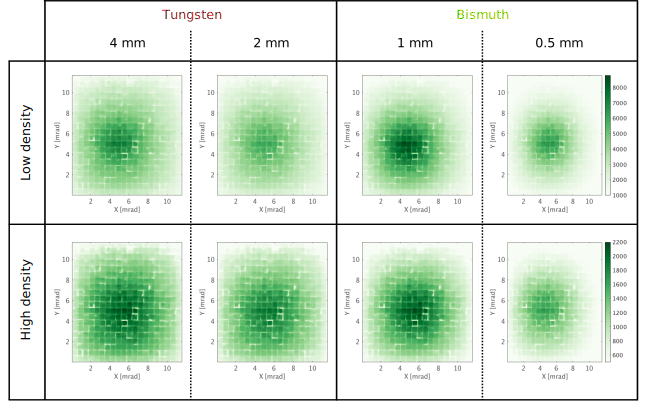
\includegraphics[trim={4.9cm 0 5cm 0}, clip, width=1.\columnwidth]{BW_GammaProfileConverter_Montage.png}

\caption[Montage of gamma profile measurements for different materials and accelerator settings.]{Montage of gamma profile images for different materials and accelerator configurations. The images on the top row are on the same colour scale, the images on the bottom respectively as well (with a maximum value of 1/4). ADD DESCRIPTION WHICH IS WHICH. TOP LOW DENSITY, BOTTOM HIGH. ALWAYS WTHICK,THIN,BITHICKTHIN, NEW ROW.}
\label{BW:figs:Gprofile_materials_montage}
\end{figure}



More specifically, $2\,\mathrm{mm}$ and $4\,\mathrm{mm}$ tungsten, $0.5$ and $1\,\mathrm{mm}$ bismuth were mounted on $0.5\,\mathrm{mm}$ plastic (PTFE), all on a motorised linear stage that allows switching between the materials or removing the converter targets from the beam path completely.
\vspace{\baselineskip}

The quantities we measure are the total counts on the gamma profile monitor (yield) and the width of the gamma signal in terms of the \textsc{fwhm} in the vertical and horizontal axis. This is being investigated for all 4 converter targets in two different electron regimes (one higher energy less charge from lower density plasma, the other higher charge but lower energy from a high density plasma). 10 shots were taken at each configuration (backing pressure A, converter 1...).


\begin{figure}
\centering
\includegraphics[trim={4.9cm 0 5cm 0}, clip, width=.9\columnwidth]{2018QED_Converter_Yield.png}
\caption[Gamma-ray yield of the bremsstrahlung source for tungsten and bismuth at different accelerator settings.]{Total measured gamma yield of the gamma-ray beam at two accelerator configurations (low and high electron densities) for tungsten (W, red) and bismuth (Bi, yellow). The values for the thin and the thick targets are shown by the thin and thick bars, respectively.}
\end{figure}


From the results we can see a couple of trends. The divergence and yield for each material is larger when the solid target is thicker, i.e. the measured gamma yield is higher for $1\,\mathrm{mm}$ of bismuth than for $0.5\,\mathrm{mm}$, and higher for $4 \,\mathrm{mm}$ than for $2\,\mathrm{mm} $of tungsten, and similarly so with respect to the divergence.
More material leads to more scattering and an increase in divergence. At the same time it indicates that more energy is converted into photons when using thicker targets.

We see that the electrons produced in a higher density plasma (higher charge, lower energy) provide a lower yield of gamma rays at higher divergences. This also appears to be sensible as the initial divergence of the electrons is higher. The yield scales quadratically with the electron energy whilst the photon number relies only linearly on the electron charge. A higher energy electron beam, even at slightly lower charge, can hence provide a higher yield.

\begin{equation}
\boxed{Bremstrahlung Energy \sim Z^2 N(E) E^2}
\end{equation}
\begin{figure}
\centering
\includegraphics[trim={4.9cm 0 5cm 0}, clip, width=.9\columnwidth]{2018QED_Converter_Divergence.png}
\caption[Divergence of the gamma-ray beam for tungsten, bismuth and different accelerator settings.]{FWHM divergence of the gamma-ray beam at two accelerator configurations (low and high electron densities) for tungsten (W, red) and bismuth (Bi, yellow). The values for the thin and the thick targets are shown by the thin and thick bars, respectively. The red line indicates the field-of-view of the collimator.}
\end{figure}

Comparing the bismuth and the tungsten targets we see that the divergence for bismuth is in general lower than for tungsten. This is probably related to the thinner target. Bismuth has a higher Z-number and can provide a similar conversion efficiency at lower scattering rates.
We also observe that the yield does not increase much more from bismuth $1\,\mathrm{mm}$ to any of the tungsten targets, whilst preserving a $\sim\,10\%$ lower divergence. This indicates that most of the electrons already transferred all or a large fraction of their energy into gamma radiation and more material mainly leads to more scattering. The yield of bismuth, on the other hand, increases by around 50 percent from $0.5$ to $1\,\mathrm{mm}$ thickness. In some instances for $0.5\,\mathrm{mm}$, a faint electron signal is observed on the spectrometer screens. This confirms that somewhere around those thicknesses most of the electron energy is converted to radiation, reaching saturation.

\SMComm{How accurately is the field of view matching. Maybe run GEANT sim on the sharpness of edges.}
\EliasComm{Does this match at all? Z=74 and 83, so the ratio is 1.25, so 25 percent more yield.}

Another result can be seen in Figure \ref{BW:figs:converter_pointing}. Here the pointing stability of the gamma signal is shown. There is some scatter but most of the targets operate at a comparable level and do not show a clear trend. This makes sense, as the general pointing mainly depends on the electron pointing and should not depend on the material.

\iffalse
\begin{figure}
\centering
\includegraphics[trim={4.9cm 0 5cm 0}, clip, width=.9\columnwidth]{2018QED_Converter_YieldVDiv.png}
\caption{Gamma Profile Yield and divergence. Maybe switch to a combined plot for x and y axis.}
\label{BW:fig:converter_yield_v_div}
\end{figure}


\begin{figure}
\centering
\includegraphics[trim={4.9cm 0 5cm 0}, clip, width=.5\columnwidth]{2018QED_GConverter_PointingMM.png}\includegraphics[trim={5cm 0 5cm 0}, clip, width=.5\columnwidth]{2018QED_GConverter_PointingSigma.png}
\caption{Left: Centroid position on detector in mm, coordinate zero point is the bottom left corner of the detector. Right: Standard deviation of pointing fluctuation from mean value in mrad. This looks a bit empty. Replace this by a bar chart?}
\label{BW:figs:converter_pointing}
\end{figure}
\fi

\begin{figure}
\centering
\includegraphics[trim={4.9cm 0 5cm 0}, clip, width=.9\columnwidth]{2018QED_GConverter_Pointing.png}
\caption[Pointing of the gamma-ray beam for the different materials and accelerator settings.]{Pointing of the gamma-ray beam at two accelerator configurations (low and high electron densities) for tungsten (W, red) and bismuth (Bi, yellow). The values for the thin and the thick targets are shown by the thin and thick bars, respectively.}
\label{BW:figs:converter_pointing}
\end{figure}


\subsubsection{Throughput Collimator for Yield}

Considering the collimator and the measured divergences of the gamma rays, we can now estimate what fraction of the gamma signal that will make it through the collimator. A more divergent beam will lose more intensity but if it comes with higher yield it might still prevail.

We will use the measured \textsc{fwhm} divergence values and model the intensity profile after a Gaussian. We will also assume perfect alignment and ignore pointing for now as it is in the same ballpark for the converters and should not depend on the material.

Bismuth at $0.5\,\mathrm{mm}$ has a lower divergence and most of its energy makes it through in terms of fraction based on the initial input, followed by 1 mm bismuth. If weighed by the total flux of photons related to that converter, the higher yield of the thicker bismuth target increases the total flux. The 2 mm thick W target provides a similar throughput (in absolute numbers) as the thin bismuth target. The thicker W target reaches close to similar levels as 1 mm of bismuth but not fully.

Based on these results 1 mm bismuth appears to be the best suited candidate for this endeavour.

\begin{figure}
\centering
\includegraphics[trim={4.9cm 0 5cm 0}, clip, width=.9\columnwidth]{2018QED_AbsTransmission_V2.png}
\caption[Estimated through collimator transmitted gamma-ray yield for different materials and accelerator settings.]{Estimated transmitted yield through the collimator assuming a field of view of 7.14 mrad at two accelerator configurations (low and high electron densities) for tungsten (W, red) and bismuth (Bi, yellow). The values for the thin and the thick targets are shown by the thin and thick bars, respectively.}
\label{BW:fig:abs_transmission}
\end{figure}


\subsubsection{Noise Considerations}

The positrons produced by the BW process are detected by the timepix3 detectors. These are sensitive to gamma rays and charged particles over a wide range of energies.  The shape of the tracks in the detector allows some events to be excluded. For example, low energy charged particles produce wiggly tracks, high energy particles or gammas produce straight tracks, the length of which provides information about the angle of incidence.  As positrons transported from the collision point enter the detectors within a specific range  of angles, this can be used to exclude some high energy events.  Events which are not excluded are “candidate events”.

Gamma rays  can interact with material in the chamber (eg the magnets, the second lead collimator) and produce positrons via the BH process that have similar characteristics (energy, angle into the chicane) so that they are indistinguishable from BW positrons on the detector.  Gammas striking the vacuum windows can also scatter into the detector at the angle corresponding to a candidate event.  

 We might expect that the number of these noise events will depend on the gamma yield, the following section examines this.... 
 \vspace{\baselineskip}


When inserting the W collimator and thick W block to reduce the noise levels, the number of gamma rays that make it to the detectors is decreased significantly. This makes it more difficult to characterise how the noise at the single particle detectors (SPDs) scales as the range is limited.

Using the same setup, we are now looking at noise events reaching the SPDs, in this case only one of the TimePix detectors\footnote{Method and numbers provided by B. Kettle looking at the TimePix and finding events that look like particles, will be called clusters.}, and how it correlates with the divergence and yield of the gamma-ray signal. Our hypothesis is that a more divergent gamma-ray beam will interact with more components and apertures in the beam path, generating radiation and particles that are closely related to the BW signal and will because of this resemblance be detected by the SPDs.
\vspace{\baselineskip}

Figure \ref{BW:figs:converter_noise_div_yield} shows a plot of the total counts on the gamma detector (yield) against the number of registered particle events or `clusters' on the TimePix detector, and how the divergence is related to those noise events.

Linear trend of yield and noise on TimePix.

W data points lie on one straight line. Bi events are parallel or lower gradient, in general less noise for comparable yields.

For each material a thicker target results in more divergence. More divergence results in more noise. This confirms the need of the collimator, W block and so on and confirms the ideas behind the setup.

Looking at yield over the number of clusters, the bismuth targets perform the best when looking at fraction of flux transmitted through the collimator.
A thinner target produces less noise and bismuth provides a decent yield.

When scaling the y-axis to the absolute flux transmitted we see again that 1 mm bismuth performs similarly well as 4 mm of tungsten in terms of transmitted flux. However, we see that the ratio of yield to noise is better for bismuth due to the lower divergence.

The collimator will cut out the more divergent parts of the beam, so the noise levels will be comparable for the materials.

Looking at Figure \ref{BW:fig:Yield_with_Coll} we see that introducing the collimator cuts down the gamma yield and subsequently also the number of noise events registered on the TimePix detector. When comparing the trend of these events with the linear relations derived from the converter analysis, we see that the yield per noise further improved as we are decreasing the divergence dramatically.


\EliasComm{Need appropriate legend for all data points or combine them.}


\begin{figure}
\centering
\includegraphics[trim={4.5cm 0 5cm 0}, clip, width=.9\columnwidth]{2018QED_Converter_YieldvNoise_V2.png}
\caption[Noise versus gamma-ray yield for tungsten (W) and bismuth (Bi).]{Noise measured on the TimePix detectors as function of the yield measured on the gamma profiles for tungsten (W, red) and bismuth (Bi, yellow). The large squares indicate results from thick, the smaller ones from thin converter targets. The gradients indicate a material-dependent noise-to-yield ratio.}
\label{BW:figs:converter_noise_div_yield}
\end{figure}

\iffalse
\begin{figure}
\centering
\includegraphics[trim={4.5cm 0 5cm 0}, clip, width=.5\columnwidth]{2018QED_SignalNoise_Transmission.png}\includegraphics[trim={5cm 0 5cm 0}, clip, width=.5\columnwidth]{2018QED_SignalNoise_AbsTransmission.png}
\caption[Noise versus gamma-ray yield for tungsten (W) and bismuth (Bi).]{Noise measured on the TimePix detectors as function of the yield measured on the gamma profiles for tungsten (W, red) and bismuth (Bi, yellow). The large squares indicate results from thick, the smaller ones from thin converter targets. The gradients indicate a material-dependent noise-to-yield ratio.}
\end{figure}
\fi

\begin{figure}
\centering
\includegraphics[trim={3.0cm 0 5cm 0}, clip, width=.9\columnwidth]{2018QED_YieldvNoise_CollIN_V2.png}
\caption[Noise as a function of gamma-ray yield with the collimator in the beam path. ]{Noise as a function of gamma-ray yield with the collimator in the beam path. The noise-yield gradients for tungsten and bismuth are indicated as comparison.}
\label{BW:fig:Yield_with_Coll}
\end{figure}


\begin{figure}
\centering
\includegraphics[trim={4.9cm 0 5cm 0}, clip, width=.9\columnwidth]{2018QED_Yield_CollIN.png}
\caption[Total measured gamma yield at two accelerator configurations (low and high electron densities) for tungsten (W) and bismuth (Bi).]{Total measured gamma yield at two accelerator configurations (low and high electron densities) for tungsten (W, red) and bismuth (Bi, yellow). In turquoise the gamma yield measured using the thick bismuth target and the collimator in the beam path. The values for the thin and the thick targets are shown by the thin and thick bars, respectively.}
\label{BW:fig:Yield_with_Coll_bar}
\end{figure}


\begin{figure}
\centering
\includegraphics[trim={4.9cm 0 5cm 0}, clip, width=.9\columnwidth]{2018QED_NoiseOverYield_CollIN.png}
\caption[Fitted gradient for Noise/Yield from Figure XX at two accelerator configurations (low and high electron densities) for tungsten (W) and bismuth (Bi).]{Fitted gradient for Noise/Yield from Figure XX at two accelerator configurations (low and high electron densities) for tungsten (W, red) and bismuth (Bi, yellow). In turquoise the gradient fitted for the data using the thick bismuth target and the collimator in the beam path.}
\label{BW:fig:Yield_with_NoiseColl_bar}
\end{figure}

\subsubsection{Summary and Decision on Material}

Best flux throughput for 1 mm bismuth. Noise is also lower although the levels will change for collimator and W block conditions.
1 mm bismuth also removes all electrons and potentially reduces noise from inside the collimator (dispersed remaining electrons).

Electron regime intermediate (low density but backing pressure had to be increased due to leak). Higher energy is more preferable than a bit more charge and higher initial divergence.

In theory, even thinner target and higher Z would be favourable (as long as all electrons are converted) but Bi is the readily available material on the periodic table.

The trends confirm that we need the collimator and W block. We also see that the yield over noise improves.

\EliasComm{I estimated 50 percent loss in transmission but it looks like it is more around a factor 10. Where is this coming from? Pointing and misalignment?}
\EliasComm{Do I need to run a Monte-Carlo simulation?}


\section{Characterisation of the Gamma Signal}

\subsubsection{Yield of gamma spectrometer and profile on the different days}


\begin{figure}
\centering
\includegraphics[trim={3cm 0 5cm 0}, clip, width=.9\columnwidth]{2018QED_GSGP_Corr.png}
\caption[Linear correlation of gamma spectrometer and profile yield.]{Gamma spectrometer yield as a function of gamma profile yield for an example run. Both correlate well linearly.}
\end{figure}


\subsubsection{Detector response in experiment}

Look at the detector response in general (without corrections)

Get a better background subtraction done to avoid a fluctuation low signal tail.

Maybe make a plot of average spectra. Do they have a slight change in peak?

It seems that despite the change in spectra, the response is not changing as much.

This means the detector is not suitable to discriminate a spectrum to such detail and also is not suitable to deduce a gamma spectrum independent of assuming its shape. Luckily bremsstrahlung is well understood. It is essential to have many reference electron shots. Also a lesson for the future to take data in between.

Simulating response of detectors using GEANT.
Monoenergetic photons in a different range and present the response curves.
\vspace{\baselineskip}


Correlating Gamma profile and spec counts. No change in response for those detectors.
Seeing that this is very linear the results from gamma profile assessment are still or again valid.
This is not useful to distinguish energies.


The produced spectrum can be simulated using the electron spectra characterised earlier. GEANT. Typical gamma spectra produced are shown in FIGURE XX. 
Show that the responses for all electron spectra is fairly similar in simulations and the resulting spectra vary mostly at a low photon level and high energies.
The response of the detector only results in small variations.
\vspace{\baselineskip}

The experimental results also show only small variations which is consistent with simulations. The systematic offset is including the viewing angle, efficiency of crystals and so on.
Does the flux vary as much as the electron charge? (for the shots with W block, collimator and converter in the correlation is washed out and there is no clear indication that these things are linked). Add some plots for that as well.
Stability of gamma flux?


\begin{figure}
\centering
\includegraphics[width=.5\columnwidth]{2018QED_ElecSpecs_examples2.png}\includegraphics[width=.5\columnwidth]{2018QED_GammaSpec_simspec2.png}
\caption[Example electron spectra and corresponding in GEANT simulated gamma spectra.]{Left: Representative extreme examples of electron spectra from one day. Right: Resulting gamma spectrum based on GEANT simulations. Maybe show an average with shaded error bars instead. Add a third electron spectrum and gamma result for the other extreme.}
\end{figure}

Add the differences from day to day somewhere as well as comparison.

\begin{figure}
\centering
\includegraphics[width=.5\columnwidth]{2018QED_ElecSpecs.png}\includegraphics[width=.5\columnwidth]{2018QED_GammaSpec_simresp.png}

\includegraphics[width=.5\columnwidth]{2018QED_GammaSpec_expresp.png}\includegraphics[width=.5\columnwidth]{2018QED_GammaSpec_Average_expsim.png}

\caption{Left: Lineouts for most electron spectra. Right: Simulated detector responses. BLeft: Experimental responses. BRight: Comparison average responses.}
\end{figure}


What is the statistical variation of the signal on each day. Use the electron spectra to put a number onto this.
Use plot of relative and absolute number of photons above a threshold. Sum them up and also sum up number times energy as indicator for high energy photons.

Provide a plot with numbers on fluctuation of number of photons to expect in total and in particular above a threshold and how that varies shot-to-shot and day by day.

Provide some plots from the GEANT simulation (visualisation).

\begin{figure}
\centering
\includegraphics[trim={4.9cm 0 5cm 0}, clip, width=.9\columnwidth]{2018QED_GSpec_Variations_V2.png}

\includegraphics[trim={4.9cm 0 5cm 0}, clip, width = 0.9\columnwidth]{2018QED_GEANT_AvGSpec_V2.png}
\caption{Variations of gamma signal for the shot days. Top: Gamma-ray yield measured and relative number of photons above 400 MeV(based on GEANT simulations using the average electron spectra measured for those days). Bottom: Average gamma spectra for different shot days. Spectral shape based on GEANT simulations using average electron spectra for those days and scaled by the relative yield measured for the days.}
\end{figure}






\section{Characterisation X-ray spectra}

The X-rays are generated by a 40ps beam heating a burn-through foil, 5um kapton with 100nm of germanium. The X-rays travelling to the interaction point traverse the plastic tape which results in a filtering of lower energy X-rays (see Figure XX for simulated spectra with and without tape). The X-ray source is characterised in experiment by a pinhole camera and a crystal spectrometer. The pinhole camera measures the source size and flux and the crystal spectrometer measures the spectrum, both from the side the foil is heated from, which means it is unfiltered.

The analysis of this data has been conducted by Cary Colgan and Brendan Kettle (Imperial College).

The spectral region measured on the three shot days, averaged over shots taken on the respective days, are shown in Figure XX. The range indicated is the range of the crystal spectrometer and the sharp fall-off on the sides indicates the end of the camera chip or of the crystal (especially on day A). The height of the spectra is indicative of the relative X-ray yield. This also correlates well with measurements taken from the pinhole camera (see Figure XX). The distinct peaks are emission lines of the material and slight spectral shifts are due to smaller calibration and alignment errors but are within few eV.
Day B and C are very consistent, whereas day A indicates a change in spectrum above 1.4 keV in terms of less pronounced emission lines and lower yield. The cut-off around 1.33 keV is due to a misalignment in the crystal.

According to lab book around 4 percent conversion from laser light into X-rays.

The relative X-ray yield is shown in Figure XX, which shows a lower yield for day A and comparable yields for days B and C.
In general the spectral shape of the emission is very stable and the fluctuations are insignificant (smaller than X percent).

The measured range relates to the emission peak in the simulated spectrum (see Figure XX). We assume that the spectrum will fall off sharply on either side of the measured interval.

\begin{figure}
\centering
\includegraphics[trim={4.9cm 0 5cm 0}, clip, width=.9\columnwidth]{BW_CSpec_Pinhole_Yield.png}
\caption{Comparison yield pinhole cameras and crystal spectrometer.}
\end{figure}




\begin{figure}
\centering

\includegraphics[trim={4cm 0 5cm 0}, clip, width=.9\columnwidth]{BW_XraySpec_Morton.png}

\includegraphics[trim={4cm 0 5cm 0}, clip, width=.9\columnwidth]{BW_XraySpec_AvDay.png}
\caption{X-ray spectra. Top: X-ray spectrum simulated by Morton REF USING \cite{Roberts1980_AWECODE} (blue) and filtered by plastic (red). Bottom: X-ray spectra measured with the crystal spectrometer for different shot days. }
\end{figure}

\begin{figure}
\centering
\includegraphics[trim={4.9cm 0 5cm 0}, clip, width=.9\columnwidth]{BW_XraySpec_AvDay_Yield.png}
\caption{Average total X-ray yield as measured by the crystal spectrometer for the different shot days normalised by the maximum X-ray yield measured. The shot-to-shot fluctuations are so small that the error bars were omitted.}
\end{figure}



\section{Impact of Spectral Fluctuations on the total BW cross section}

Relate measured quantities to the cross section for the BW process.

Based on the measured X-ray spectrum (measured and simulation), estimated fluctuation of the gamma spectrum and the known remaining experimental conditions, by how much does the cross section vary on a daily basis (including charge, flux etc.).

\begin{figure}
\centering
\includegraphics[width=.5\columnwidth]{BWxsection2.png}\includegraphics[width=.5\columnwidth]{BWxsection_2D.png}
\caption{BW cross section at a fixed and variable X-ray photon energy.}
\end{figure}

\begin{figure}
\centering
\includegraphics[trim={4.9cm 0 5cm 0}, clip, width=0.8\columnwidth]{BWXsec_Angles_MortonRawYieldCorr.png}

\includegraphics[trim={4.9cm 0 5cm 0}, clip, width=0.8\columnwidth]{BWXsec_Angles_MortonCorrYieldCorr.png}

\includegraphics[trim={4.9cm 0 5cm 0}, clip, width=0.8\columnwidth]{BWXsec_Angles_AvDay.png}
\caption{Xsec fluctuation for different angles and including plastic or not Morton or not. Morton full, Morton corr plastic, measured spectrum.}
\end{figure}



The number of pairs produced from BW scales something like this

\begin{equation}
\boxed{N_{BW, day}|_{theta} \sim \int \frac{N_{ph, X}}{\mathrm{d}E_{X}} \frac{N_{ph, \gamma}}{\mathrm{d}E_{\gamma}} \sigma_{BW} (E_{X}, E_{\gamma}, \theta) \mathrm{d}E_{\gamma}\mathrm{d}E_{X}}
\end{equation}

The main angle between the two sources is about 140 degrees (XX ERROR ON THIS?). However, in general we have to fold in the angular distribution of both photon sources. The collimator has a field of view of $7.14 \pm 0.1 \,\mathrm{mrad}$ or $\pm 0.2^\circ$ from the main axis. The main contribution of angular spreads comes from the X-ray source.

The closer the angle is to a head-on collision the more the peak of the cross-section shifts towards lower gamma energies. 
If the X-ray spectrum is mainly centred around 1.5 keV and lower energies are suppressed the additional 800 MeV does not have a significant impact.
If the full X-ray spectrum (for instance Morton simulations) are included then a large pool of X-rays are available at lower energies to be paired up with the high energy photons of 600-800 MeV. We see the effect of this in Figure XX showing the fluctuation of the number of expected pairs on the days based on different angles. The differences flatten out.

The X-ray yield was higher on the XXth whilst the gamma yield and energy was higher on the 6th. These fluctuations balance each other out and the collisional geometry further mitigates the fluctuation.

\SMComm{The point you are trying to make is excellent..  but I don’t think it’s clear....

There is significant fluctuation in the gamma spectrum from day to day

But this is mainly in the high energy tail of the gammas

To calculate the effect of this you need to take into account which photon photon collisions are most likely to produce pairs.  

This depends on the invariant mass of the collision (formulae based on two energies and angle in lab frame) and is just above the threshold sqrt(s) = 2 m

You can calculate the most probably part by considering the angle of collision (40 degrees? I think  you mean 130? , as 180 would be head on).  For simplicity you ignore angular spread of both photon sources.  

The higher energy gamma rays present on some days   can produce pairs with lower energy X-ray photons, however these don’t reach the collision point as they are absorbed in the plastic on which the foil is mounted.  

As a result, the level of fluctuation in pair yield from day to day (and shot to shot) is suppressed.  
}

\iffalse
\section{Future Outlook: A gamma spectrometer to discriminate high energy photons}

Here some ideas and simulations on how to improve the gamma spectrometer design to determine the spectrum more accurately.

\subsubsection{Explanation why detector is not sensitive to the changes seen in the simulated spectra}


Show that the problem is the following:
above 10's of MeV the cross section for pair production increases and is relatively flat over long time. What happens is that gammas convert into electrons which convert into gammas in showers and so on. In most cases a high number of low few MeV gamma rays is present and the main indicator for the initial energy is how many times these showers continue to proceed and where they deposit energy. Most spectra convert to an almost exponential shower of particles and radiation, which means that most of the deposited energy from different energy gamma rays will be deposited through similar radiation. Resolving a low number of higher energy photons will be difficult as large fraction of the energy deposited will be identical to other energies.
\vspace{\baselineskip}

Show cross sections.

Show investigations in GEANT:

- looked at the experimental setup in GEANT and measured for different input energies at different parts of the spectrometer the radiation and particle spectra

Compton scattering also does not work anymore due to sensitivities (lower energies see \cite{Corvan2014_Gamma}).

\begin{figure}
\centering
\includegraphics[width=.9\columnwidth]{CsI_MassAttenuation.png}
\caption{Mass attenuation coefficient for CsI shows it becomes quite flat at hundreds of MeV just producing pairs. This is from a presentation and I would have to plot this myself probably again. All the data is on the NIST though.}
\end{figure}


\subsubsection{Present Ideas on how to improve the detector}

Ideas: 

- insert different materials at various positions (one part of the spectrometer measures the main part of the spectrum, a part further in only shows energies above a threshold?)

- use magnets either as pair spectrometers (see Gianluca's design) or ...

- ... to `clean up' the signal by removing generated pairs from the system (requires a lot of space)

- should stay compact
\vspace{\baselineskip}

First results did not look promising. The low number of high energy particles etc. is really swamped by other signals.
To really make a difference one would have to kick out low energy particles several times. From experience I can not just put one big magnet around the spectrometer as the magnetic field will affect the scintillators.
Using Gianluca's pair spectrometer is also not feasible as for a compact version of this design the higher energies will not be deflected sufficiently and the number of particles is very low, will be swamped by other signal.

Use gamma profile as converter or even the vacuum window (less divergence) and then disperse. Having the pair measurements and the array response will constrain the spectrum. 


\begin{figure}
\centering
\includegraphics[width=.9\columnwidth]{CombinedSpecSketch.png}
\caption{Combined design.}
\end{figure}
\fi



\section{Results of the Breit-Wheeler Analysis}


\subsubsection{Discussion of how this work fits in the big picture of the complete BW analysis}
\EliasComm{Here a brief discussion of the findings of the BW analysis, mainly focusing on individual components that worked like SPD, chicane, tracking, background-suppression, X-ray source, gamma source and shown mitigation, calibration.}

How extensive?

Described most of the setup and the different diagnostics.

Maybe:

... reiterate the setup and the different components.

... emphasise that we have seen from the analysis that the gamma and X-ray sources were working...

... and that the diagnostics were working as well.

... explain that the single particle diagnostics were behaving in an expected way and we investigated their behaviour using

... the tungsten blob shots

... the magnet chicane (tracking)

... noise behaviour with different blocks in.

... mention that we see a number of events on each shot based on Bethe-Heitler...

... and there are some events above that expected background

... these events are particularly visible on the 6th where the gamma conditions and the alignment was working properly.



\section{Conclusion}

Electron beams from LWFA underlie intrinsic fluctuations and the performance of the accelerator can vary from day to day.

There are, broadly speaking, four avenues to account for these fluctuations within this experiment layout: 

Firstly, attempt to decrease the fluctuations and stabilise the electron source.

Secondly, choose a conversion process that mitigates the fluctuations of the electron source.

Thirdly, if after additional stability and mitigation the source still fluctuates significantly, we have to attempt measuring the fluctuations.

Finally, if we are not able to measure the fluctuations on-shot we can identify the range of the fluctuations and mitigate their impact on the total cross-section by tailoring the X-ray source (angle, cut-off in spectrum). This reduces the total cross-section but mitigates fluctuations.



A comment about designing your experiment such that parts of the X-ray spectrum we can not measure are being blocked by material such that the gamma components we can not resolve are not impacting on the cross section. The angle is also a handle on equalising the cross section across the window of gamma energies such that few high energy photons still access the same pool of photons and the cross section is low.

Flaw of wakefield accelerator are the intrinsic fluctuations of the electron beam. Better stability by improving the e-beam but for instance by using bremsstrahlung we already cut out some of the uncertainty. See simulations that show that fluctuations in the spectral shape are not impacting the overall gamma spectrum much. 
If we now tailor the X-rays accordingly and choose the angle of the collision appropriately we can mitigate the impact of these fluctuations (maybe at a marginal cost of produced positrons) and have more stable conditions at the experiment.



... decide whether this would be just RR or if it actually would make sense to do this for a BW setup as well to round things off.
Most of the diagnostics would work both ways.

.. however, the BW setup does not require an a0 measurement and dual-axis resolution. The important part could be the improved spectral measurement, but if we mitigate the targetry, this would be okay. Maybe we can argue that the setup is already quite complicated. Here it would be better to leave the back-end constant (shielding and noise is a sensitive issue), but improve the signal by using more charge (could consider shock injection if the control is better as the charge is much higher than in the case of self- and ionisation injection PROVIDE SOME NUMBERS FROM LINEAR ICS AS DIRECT COMPARISON).

.. mitigate effects:

... X-rays can only be measured in a narrow window (700eV), so cut out the signal under the measurement as before using plastic tape

... measure spectrum and source from interaction point side?

... above we need to be sure how the spectrum behaves. It is hard to cut above but not below.

... a second X-ray camera to measure a part of the higher energy spectrum. Would it be enough without overlap (can't do overlap unfortunately...), would there be an issue with higher orders?

... is resolution or range more important? How much further away would we have to be to measure the full range?

... is the range of angles a problem? If so, can we add a spatial collimator also for the tape target (would produce noise again...)

